\section{Environment plug-in}

\subsection{Overview}

The architecture of the plug-in comes from \cite{DeclarativeArchitecture}, to
provide an intuitive way of building an environment: by drawing features on a
map. The most difficult part in this approach is that intersecting features are
allowed and should give a result consistent with user expectations.

As a starting point, we focused on generating a height map, using the concepts
from \cite{FeatureTree}. It had the advantage of being able to merge features
smoothly whenever they intersect, rather than using the more convoluted
conflict-resolution mechanism of \cite{DeclarativeArchitecture}.

\bigskip

The basic unit managed by this plugin is a \emph{feature}, which lies in a
certain area, has a certain height profile and knows how to interact with the
other features that may intersect it. From the collection of all the features
drawn on the map by the user it builds a tree encoding how to build the final
height map by successively merging sets of features together.
%TODO: mention models (e.g. trees for forests)


\subsection{Features}

\subsubsection{Mountains}

Our first implementation of the Mountain feature corresponded to what is presented in \cite{FeatureTree}. However, the 2D random functions we tried did not yield satisfying results. That's why we switched to another version, where we import at random a part of a heightmap taken from a website \cite{terrain-party}. This website import the heightmaps through satellite imaging.

\subsection{Graphical User Interface (GUI)}

A picture of the interface is presented in Fig.~\ref{fig:env-gui1}. Using the interface, the user can choose the feature he wants to draw. He can then draw it using a pencil integrated in Blender, drawing polygons here. After having completed the drawing of the features, the user can ask for the generation of the environment. It can then hide the polygons, and also modify parameters that are feature-specific.

\begin{figure}
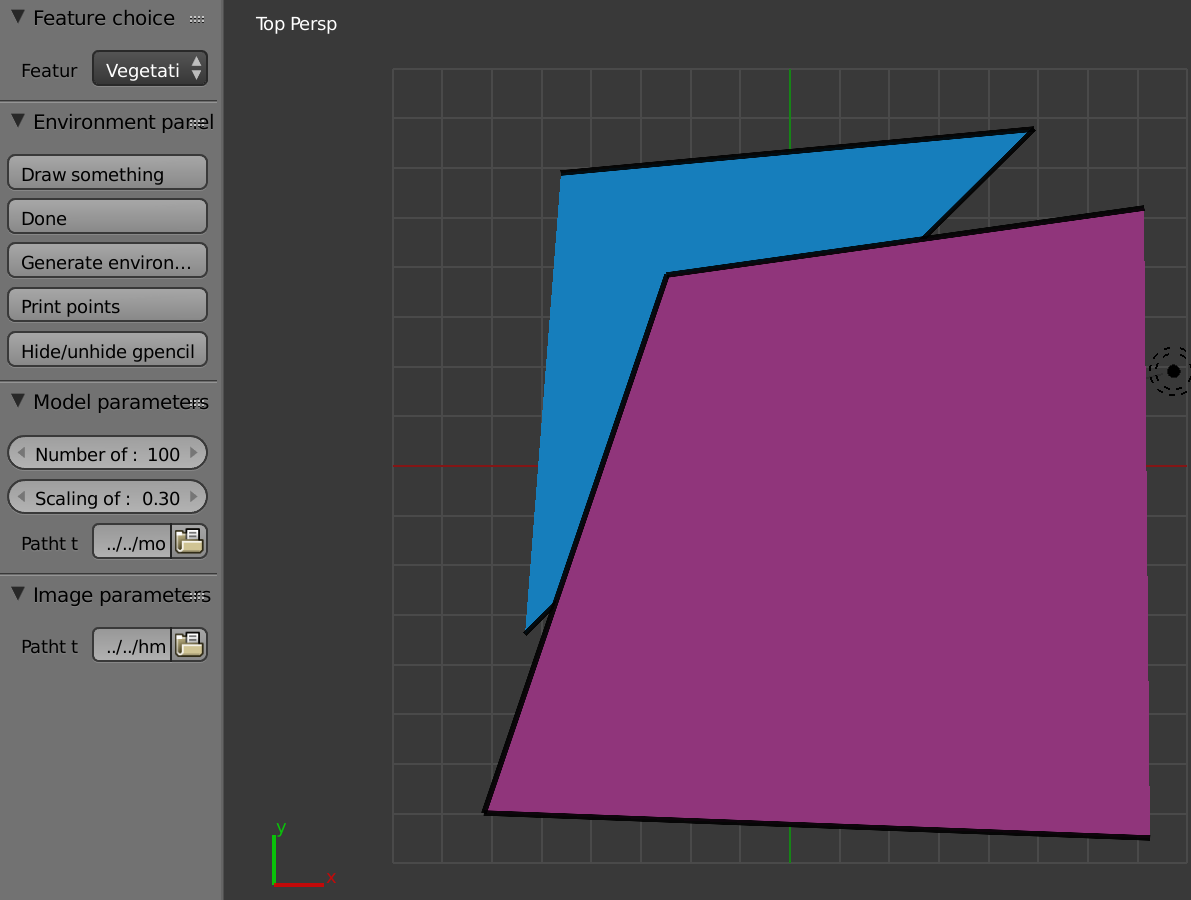
\includegraphics[width=\textwidth]{img/env_gui1.png}
\caption{GUI of the Environment plug-in, with two features (in blue and magenta)}
\label{fig:env-gui1}
\end{figure}

